\documentclass[12pt,superscriptaddress,preprint,nofootinbib,aps,prd]{revtex4-2}

% Core packages
\usepackage[utf8]{inputenc}
\usepackage{amsmath,amssymb,mathtools}
\usepackage{graphicx}
\usepackage{xcolor}
\usepackage{url}
\usepackage{enumerate}
\usepackage{cancel}
\usepackage{tikz}
\usetikzlibrary{positioning,arrows}
\usepackage{tikz-cd}
\usepackage[title]{appendix}
\usepackage{siunitx}
\sisetup{per-mode=symbol}
\usepackage{mathrsfs}
\usepackage{import}
\usepackage{enumitem}
\usepackage{booktabs}

% ----------------------------------------------------------------------------
% Submission-oriented edits (no red/blue issue text in compiled output)
% ----------------------------------------------------------------------------
\newcommand{\RCred}[1]{#1}
\newcommand{\RCblue}[1]{}
% January 2026 referee update pass: edits are marked in blue via \EDIT{...}
\newcommand{\EDIT}[1]{\textcolor{blue}{#1}}

% Units
\DeclareSIUnit\au{a.u.}
\DeclareSIUnit\angstrom{\text{\AA}}

% Hyperref must remain last
\usepackage[bookmarks,linktocpage,pdfpagelabels,plainpages=false,
hyperfigures,linkcolor=blue,citecolor=blue]{hyperref}
\hypersetup{colorlinks=true}

% Ensure compatibility with apsrev4-2 .bbl helper macros
\makeatletter
\let\href@noop\relax

% Fix TOC spacing for Roman numerals (compatible with revtex4-2)
\renewcommand*\l@section{\@dottedtocline{1}{0em}{3em}}
\renewcommand*\l@subsection{\@dottedtocline{2}{1.5em}{4em}}
\renewcommand*\l@subsubsection{\@dottedtocline{3}{3.5em}{5em}}
\makeatother

% Theorem environments
\newtheorem{theorem}{Theorem}[section]
\newtheorem{lemma}[theorem]{Lemma}
\newtheorem{axiom}[theorem]{Axiom}
\newtheorem{proposition}[theorem]{Proposition}
\newtheorem{corollary}[theorem]{Corollary}
\newtheorem{definition}[theorem]{Definition}
\newtheorem{remark}[theorem]{Remark}
\newtheorem{observation}[theorem]{Observation}
\newtheorem{conjecture}[theorem]{Conjecture}

% Proof environment
\newenvironment{proof}[1][Proof]{\noindent\textit{#1.} }{\hfill$\square$\par\medskip}

% Macros
\newcommand{\Rec}{\mathrm{Recognition}}
\newcommand{\N}{\mathbb{N}}
\newcommand{\NN}{\mathbb{N}}
\newcommand{\id}{\mathrm{id}}
\newcommand{\Id}{\mathrm{id}}
\newcommand{\Post}{\mathsf{Post}}
\newcommand{\RR}{\mathbb{R}}
\newcommand{\ZZ}{\mathbb{Z}}

% Footnote style
\renewcommand{\thefootnote}{\fnsymbol{footnote}}

% Section and subsection numbering format (I, II, III for sections; II.1, II.2, etc. for subsections)
\makeatletter
% Save class defaults so \appendix can label appendices (A, B, ...) correctly.
\let\RC@origthesection\thesection
\let\RC@origthesubsection\thesubsection
\makeatother
\renewcommand{\thesection}{\Roman{section}}
\renewcommand{\thesubsection}{\thesection.\arabic{subsection}}
\makeatletter
\renewcommand{\p@subsection}{} % Prevent double section number in \ref (fixes §II II.1 issue)
\makeatother

\begin{document}

\title[Toward a Discrete Informational Framework for Classical Gravity]{\texorpdfstring{Toward a Discrete Informational Framework for Classical Gravity: \\
Foundations, Constraints, and Testable Predictions}{Toward a Discrete Informational Framework for Classical Gravity: Foundations, Constraints, and Testable Predictions}}

\author{Jonathan Washburn}
\email{washburn@recognitionphysics.org}
\affiliation{Recognition Physics Institute, Austin, Texas, USA}

\author{Megan Simons}
\affiliation{Recognition Physics Institute, Austin, Texas, USA}

\author{Elshad Allahyarov}
\email{elshad.allakhyarov@case.edu}
\affiliation{Recognition Physics Institute, Austin, Texas, USA}
\affiliation{Institut f\"ur Theoretische Physik II: Weiche Materie, Heinrich-Heine Universit\"at D\"usseldorf,
Universit\"atsstrasse 1, 40225 D\"usseldorf, Germany}
\affiliation{Theoretical Department, Joint Institute for High Temperatures, Russian Academy of Sciences (IVTAN),
13/19 Izhorskaya street, Moscow 125412, Russia}
\affiliation{Department of Physics, Case Western Reserve University, Cleveland, Ohio 44106-7202, United States}

\begin{abstract}
\EDIT{We present a discrete informational (``ledger'') framework for classical gravity and a fixed modified-gravity response kernel (Information-Limited Gravity, ILG). In the cost-first formalization, a d'Alembert-type Recognition Composition Law uniquely forces the cost functional $J(x)=\frac12(x+x^{-1})-1$ and yields a forcing chain (Logic$\to$MP$\to$Discreteness$\to$Ledger$\to$Recognition$\to$Unique $J$$\to$Golden ratio$\to$Eight-tick$\to D{=}3) as necessary consequences. In the quasi-static weak-field limit this enforces a scale- and time-dependent response $w(k,a)=1+C\,X^{-\alpha}$ with $X:=k c\tau_0/a$, exponent $\alpha=\tfrac12(1-\varphi^{-1})\approx 0.191$, and amplitude $C=\varphi^{-3/2}\approx 0.486$. In real space the modification corresponds to a nonlocal Green's function with point-source scaling $\delta\Phi(r)\propto r^{\alpha-1}$ (and hence $w(r)-1\propto (r/r_0)^\alpha$ in the scaling regime), while disk-galaxy predictions require a convolution over baryonic surface densities. We confront the scaling-form kernel with galaxy rotation curves (SPARC) and identify coupled falsifiers across weak lensing, large-scale structure, and gravitational-wave dispersion. We also highlight an updated zero-parameter closure on the astrophysics side: the stellar mass-to-light ratio is derived as $M/L\simeq\varphi$ (solar units), removing a leading nuisance parameter in rotation-curve analyses. We distinguish certificate-backed claims (Lean certificate surface) from optional heuristic motivations (e.g.\ fractional-memory/latency) retained only for intuition.}
\end{abstract}

\maketitle

\tableofcontents

%=============================================================================
\section{Introduction}
\label{sec:intro}
%=============================================================================

\subsection{Motivation and Context}

Unifying general relativity \cite{einstein1916,MTW1973} with quantum mechanics \cite{dirac1930,dewitt1967} remains a central challenge in theoretical physics. Despite GR's empirical success at classical scales \cite{wald1984,will1993}, a consistent quantum theory of gravity is elusive. This has motivated exploring discrete spacetime structures \cite{wheeler1990,rovelli2004,penrose1971,thooft1993}---loop quantum gravity \cite{rovelli2004,ashtekar2004}, causal sets \cite{bombelli1987,sorkin2003}, Regge calculus \cite{regge1961}, and related programs \cite{konopka2006}. Information-theoretic perspectives \cite{bekenstein1973,hawking1975,thooft1993,susskind1995,maldacena1999,wheeler1990} inspire emergent-gravity proposals \cite{verlinde2011,padmanabhan2010,jacobson1995}, though most lack falsifiable predictions at accessible scales.

Astrophysically, $\Lambda$CDM successfully explains large-scale structure \cite{planck2018,bennett2003} but encounters persistent galactic-scale tensions: core-cusp discrepancies, missing satellites, and too-big-to-fail problems \cite{bullock2017,weinberg2015,moore1999,klypin1999,boylankolchin2011}. MOND \cite{milgrom1983} empirically fits rotation curves \cite{famaey2012,mcgaugh2016,lelli2017} yet lacks fundamental theoretical underpinnings and struggles with cluster-scale observations \cite{clowe2006,sanders2003}. This situation motivates exploring whether galactic dynamics might offer empirical handles on discrete quantum-gravity structures.

\subsection{Main Results}

This paper presents three key advances:

\paragraph{(1) Cost-first forcing chain and uniqueness.}
\EDIT{Starting from the cost of recognition events, a d'Alembert-type Recognition Composition Law yields a forcing chain: logic emerges from cost minimization, the Meta-Principle is derived (not postulated), discreteness and ledger structure are forced, and $\varphi$, the minimal eight-tick cycle, and $D=3$ follow as necessary consequences. This upgrades the foundation from heuristic motivation to a uniqueness-driven derivation.}

\paragraph{(2) Fixed ILG kernel and derived parameters.}
\EDIT{In the quasi-static weak-field regime, the forced structure induces a fixed response kernel $w=w(X)$ with $X:=k c\tau_0/a$ and
$w(k,a)=1+C\,X^{-\alpha}$, where the exponent is the RS-canonical value $\alpha=\tfrac12(1-\varphi^{-1})\approx 0.191$ and the canonical amplitude is $C=\varphi^{-3/2}\approx 0.486$. The $X$-only structure yields reciprocity diagnostics linking scale and time dependence in matched $(k,z)$ bins.}

\paragraph{(3) Empirical confrontation and falsifiers (rotation curves and beyond).}
\EDIT{We confront the scaling-form kernel with galaxy rotation curves (SPARC) and centralize falsifiers in lensing, large-scale structure, and gravitational-wave dispersion. In parallel with the kernel derivation, the astrophysical calibration is strengthened: the stellar mass-to-light ratio is derived as $M/L\simeq\varphi$ (solar units), removing a leading nuisance parameter from rotation-curve analyses and tightening the falsification surface.}

\subsection{Approach and Framework}

\EDIT{We organize the framework in two layers. The \emph{cost-first} layer treats the cost/defect functional as primitive and proves (i) logic as the structure of cost minima and (ii) the Meta-Principle as a derived theorem because the defect diverges as $x\to 0^+$ (Theorem~\ref{thm:MP}). For narrative continuity we still refer to this derived statement as MP. Combined with structural constraints---locality, integrality, conservation, and minimality---this forces a discrete double-entry bookkeeping system with integer postings on directed edges, atomic ticks, and closed-chain neutrality (a discrete Kirchhoff law). The unique symmetric cost functional used throughout is $J(x) = \frac{1}{2}(x + x^{-1}) - 1$ (Theorem~\ref{thm:unique-cost}). Discrete exterior calculus (DEC) provides a bridge to continuum Poisson equations in appropriate limits, while synchronization constraints select the minimal eight-tick cycle and (in the stated hypothesis class) $D=3$.}

\subsection{Key Distinguishing Features}

\paragraph{Derived functional form vs.\ phenomenological ansatz.} \EDIT{Most modified-gravity proposals introduce fitted functions with adjustable parameters. Here the scaling-form ILG kernel is treated as a forced consequence of the cost-first ledger structure: a uniqueness theorem fixes the cost functional, and the resulting forcing chain fixes $\varphi$, the eight-tick cycle, and the kernel exponent $\alpha=\tfrac12(1-\varphi^{-1})$. The ``fractional memory / latency'' narrative provides useful intuition for why a power-law response is natural, but it is not the foundational derivation.}

\paragraph{Informational foundation vs. geometric ansatz.} Unlike loop quantum gravity or causal sets, which impose discrete geometric structures \emph{a priori}, the ledger framework constrains discrete structure from a minimal informational axiom. Unlike emergent-gravity proposals (Verlinde, Jacobson), which remain qualitative, the ledger program yields quantitative, falsifiable predictions.

\paragraph{Machine-checkable proofs.} \EDIT{Core claims used by this paper are supported by Lean 4 certificates (a certified import-closure) rather than informal derivations. The broader monolith contains additional modules still under development; accordingly, we scope ``proved'' claims to the specific certificate surface referenced by this paper and its companion audit paper.}

\subsection{Current Status and Scope}

The paper presents a complete derivation chain with identified gaps. We distinguish three claim tiers:

\begin{center}
\small
\begin{tabular}{p{0.28\linewidth}p{0.22\linewidth}p{0.44\linewidth}}
\toprule
\textbf{Component} & \textbf{Status} & \textbf{Outstanding Work} \\
\midrule
\EDIT{Cost uniqueness (T5)} & \EDIT{Certified} & \EDIT{Narrative integration and exposition for non-formal readers.} \\
\EDIT{$\varphi$, eight-tick, $D=3$ (necessity pipeline)} & \EDIT{Certified (scoped)} & \EDIT{Independent review; broader hypothesis-class discussion.} \\
\EDIT{ILG kernel exponent $\alpha$ and amplitude $C$} & \EDIT{Certified} & \EDIT{Finalize the mapping between kernel conventions across galaxy/cosmology sections.} \\
\EDIT{$\lambda_{\mathrm{rec}}$ identity / derivation} & \EDIT{Certified (scoped)} & \EDIT{Strengthen the presentation of the curvature-functional derivation; connect to audit interfaces.} \\
\EDIT{$M/L\simeq \varphi$ (astrophysical closure)} & \EDIT{Certified} & \EDIT{Propagate into all empirical pipelines (SPARC, lensing) with public artifacts.} \\
\EDIT{Fractional-memory/latency mechanism} & \EDIT{Heuristic / optional} & \EDIT{Retained only as intuition; not required for the cost-first derivation.} \\
\EDIT{SPARC fits} & \EDIT{\textbf{Verified}} & \EDIT{Robustness checks and a fully convolutional disk calculation.} \\
\bottomrule
\end{tabular}
\end{center}

\textbf{Critical dependencies:} \EDIT{the remaining work is primarily (i) editorial: making the cost-first forcing chain legible to the physics community; (ii) computational: completing the full convolution-based disk prediction and publishing end-to-end reproducibility artifacts; and (iii) scope discipline: ensuring all ``proved'' claims in this manuscript correspond to the referenced certificate closure (rather than the entire monolith).}

\paragraph{Scope of empirical claims.} \EDIT{For comparability with the literature, parts of the SPARC analysis are presented in a ``fit-first'' style (treating $(A,\alpha,r_0)$ as free). The theory fixes the exponent $\alpha$ (and canonical amplitude $C$) via the forcing chain, and derives $M/L \simeq \varphi$ (solar units). This tightens falsifiers: (i) mechanism-specific signatures (constant slope and $X$-reciprocity), (ii) weak-lensing modifications at 1--10 Mpc (LSST/Euclid), (iii) $k$-resolved large-scale structure tests (DESI/Euclid), and (iv) GW dispersion audits. The companion audit paper develops BRST-consistent quantum completion interfaces and certificate-traceable audit envelopes.}

\subsection{Organization}

\EDIT{Section~\ref{sec:model} presents the ledger framework: the cost-first/forcing-chain framing, axioms, structural results (summary), the DEC bridge, and the kernel statement (with optional fractional-operator intuition deferred to an appendix). Section~\ref{sec:results} reports SPARC fits, Bayesian model comparison, and conditional predictions. Section~\ref{sec:discussion} interprets results, catalogs remaining open issues, and outlines observational/theoretical extensions. Section~\ref{sec:conclusions} summarizes. Appendices provide theorem derivation sketches, proof/audit pointers, units-quotient challenges, synchronization certificates, and fractional-operator details.}

\subsection{Reader's Guide (Dependency Chain)}

To make the logical dependencies explicit, the core narrative is:
\begin{itemize}[itemsep=1pt]
  \item \EDIT{\textbf{Cost $\to$ logic/MP $\to$ structure:} the cost-first layer yields logic-from-cost and MP as a derived constraint (Theorem~\ref{thm:MP}), which forces discrete ledger structure and a unique cost functional (Theorem~\ref{thm:unique-cost}).}
  \item \EDIT{\textbf{Structure $\to$ constants and scaling:} self-similarity pins $\varphi$ and the minimal eight-tick cycle, fixing the ILG exponent $\alpha$ and canonical amplitude $C$ at the kernel level.}
  \item \EDIT{\textbf{Bridge to continuum:} DEC connects the discrete ledger cost to a Poisson-limit description and clarifies how the nonlocal response is implemented as a Fourier multiplier / Green-function convolution.}
  \item \EDIT{\textbf{Optional intuition:} the scale-free latency $\to$ fractional-memory story provides heuristic motivation for why power-law response is natural, but it is not the foundational derivation.}
  \item \EDIT{\textbf{Kernel $\to$ data tests:} we confront the kernel with SPARC rotation curves and centralize cross-probe falsifiers (lensing, LSS, GW dispersion), strengthened by the derived $M/L\simeq\varphi$ closure.}
\end{itemize}

%=============================================================================
\section{The Model}
\label{sec:model}
%=============================================================================

\paragraph{Section Roadmap.} \EDIT{We construct the framework in four logical stages (separating the cost-first derivation from optional heuristic intuition):}
\begin{enumerate}[label=(\roman*), leftmargin=1.5em, itemsep=0pt]
    \item \EDIT{\textbf{Cost-first foundations (\S\ref{subsec:notation}--\S\ref{subsec:theorems-summary}):} we present the MP/ledger setup and the uniqueness of the cost functional $J$ (T5), together with the forcing chain that pins $\varphi$, eight-tick, and $D=3$ (in the stated hypothesis class).}
    \item \EDIT{\textbf{Continuum bridge (\S\ref{subsec:continuum}--\S\ref{subsec:mass}):} we map the discrete ledger to continuum physics via DEC and recover the Poisson limit.}
    \item \EDIT{\textbf{ILG kernel (\S\ref{subsec:ilg-derivation}):} we state the fixed scaling-form kernel $w=w(X)$ and its reciprocity diagnostics; the scale-free latency $\to$ fractional-memory story is optional intuition, not the foundational derivation.}
    \item \EDIT{\textbf{Parameter fixing and identities (\S\ref{subsec:constraints}):} we collect the derived values of $\alpha$ and $C$ (and related identities such as $\lambda_{\mathrm{rec}}$) and state the empirical falsifiers.}
\end{enumerate}

\paragraph{Logical Structure.} \EDIT{The optional latency/fractional-memory intuition is summarized below for interpretive context; the cost-first forcing chain is the primary derivation.}
\begin{center}
\small
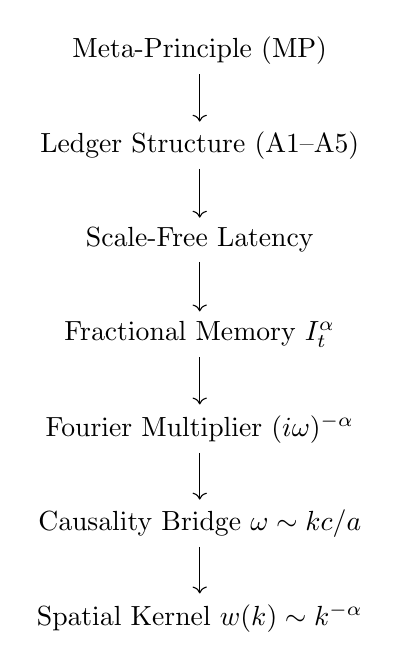
\begin{tikzpicture}[node distance=1.2cm]
  \node (Axiom) {Meta-Principle (MP)};
  \node (Ledger) [below of=Axiom] {Ledger Structure (A1--A5)};
  \node (Latency) [below of=Ledger] {Scale-Free Latency};
  \node (Fractional) [below of=Latency] {Fractional Memory $I_t^\alpha$};
  \node (Fourier) [below of=Fractional] {Fourier Multiplier $(i\omega)^{-\alpha}$};
  \node (Causality) [below of=Fourier] {Causality Bridge $\omega \sim k c/a$};
  \node (Kernel) [below of=Causality] {Spatial Kernel $w(k) \sim k^{-\alpha}$};
  
  \draw[->] (Axiom) -- (Ledger);
  \draw[->] (Ledger) -- (Latency);
  \draw[->] (Latency) -- (Fractional);
  \draw[->] (Fractional) -- (Fourier);
  \draw[->] (Fourier) -- (Causality);
  \draw[->] (Causality) -- (Kernel);
\end{tikzpicture}
\end{center}
\noindent \EDIT{\textit{(Note: This diagram summarizes the optional fractional-memory/latency intuition discussed in Appendix~\ref{app:fractional} and \cite{washburn2024fractional}. The cost-first forcing chain is the primary derivation; this latency path is retained only as intuition for why a power-law response is natural.)}}

\subsection{Notation and Conventions}
\label{subsec:notation}

\paragraph{Recognition events.} We postulate that physical processes can be modeled as sequences of \emph{recognition events}---discrete occurrences in which information is exchanged between localized degrees of freedom. In the gravitational context, an operational interpretation is provided by \emph{ledger closure}: a recognition event corresponds to closing a ledger transaction (balancing accounts). Unclosed transactions constitute a backlog with power-law persistence, manifest observationally as the ILG kernel. \RCred{The precise physical interpretation in other contexts (measurement events, interactions, decoherence) and the connection to quantum measurement theory remain open} \RCblue{[TODO: Extend operational definition beyond gravity; specify recognition criteria for quantum systems; design direct experimental test]}. The framework constrains the mathematical structure of recognition sequences via the ledger axioms.

\paragraph{Discrete variables.} We adopt the following notation:
\begin{itemize}[itemsep=2pt]
  \item \textbf{Discrete anchors:} Temporal and spatial units $(\tau_0, \ell_0)$ represent tick duration and maximal spatial advance per tick in the discrete model. These are dimensionless scaffolding parameters; physical predictions depend only on invariant ratios extracted via the units quotient (Appendix~\ref{app:units}).
  \item \textbf{Postings and potentials:} Integer-valued 1-forms $w: E \to \ZZ$ on directed edges; potentials $\phi: V \to \ZZ$ on vertices. When circulation vanishes on all cycles, $w = \nabla\phi$.
  \item \textbf{Cost functional:} $J(x) = \frac{1}{2}(x + x^{-1}) - 1$ for $x > 0$, chosen (and later justified) to satisfy analyticity, symmetry $J(x) = J(x^{-1})$, convexity, and normalization $J(1) = 0$, $J''(1) = 1$.
  \item \textbf{DEC conventions:} Cochains on $k$-cells: 0-cochains on vertices, 1-cochains on edges. Coboundary operator $d$ satisfies $d \circ d = 0$.
  \item \textbf{Continuum limits:} Limits $\Delta t, \Delta x \to 0$ with $\Delta x / \Delta t \to c$ under standard mesh regularity.
  \item \EDIT{\textbf{Golden ratio:} $\varphi := (1+\sqrt{5})/2 \approx 1.618$ is treated as a forced constant (pinned by self-similarity) rather than a conjectural input.}
\end{itemize}

\subsection{The Recognition Axiom and Ledger Structure}
\label{subsec:axiom}

\EDIT{In the cost-first formalization, MP is a derived theorem (T1) rather than an additional axiom; we state it explicitly here to keep the ledger construction readable.}

\begin{theorem}[T1: Meta-Principle (MP) (derived)]
\label{thm:MP}
\EDIT{(Derived statement; historically presented as an axiom.)}
A recognition event requires non-empty data:
\begin{equation}
  \mathrm{MP} := \neg \exists\, \Rec(\emptyset, \emptyset).
\end{equation}
\end{theorem}

\EDIT{This statement rules out the ``null event'': the empty set cannot ``recognize'' the empty set. It is intentionally minimal; it constrains admissible discrete structures without determining physics \emph{a priori}.}

Interpreting physical evolution as a sequence of recognition events, we construct a \emph{ledger calculus}. We adopt the following axiom system:

\begin{description}[labelwidth=3.4cm,leftmargin=3.6cm,itemsep=1pt]
    \item[Axiom A1 (Non-triviality).] Every tick carries at least one non-zero posting.
    \item[Axiom A2 (Locality).] Postings occur only between ordered vertex pairs.
    \item[Axiom A3 (Integrality).] Posting magnitudes are integers, capturing quantized ledger entries.
    \item[Axiom A4 (Conservation).] Any closed subsystem conserves total postings: inflow equals outflow.
    \item[Axiom A5 (Minimality).] Temporal resolution is maximally fine-grained; each tick carries exactly one atomic posting.
\end{description}

The collection (A1)--(A5) defines the ledger calculus. Theorem~\ref{thm:MP} motivates A1; A2--A5 encode locality, discreteness, conservation, and minimal structure.

\subsection{Gödel dissolution (no self-reference)}
\label{subsec:godel}
\EDIT{A foundational consistency safeguard is \emph{Gödel dissolution}: within the cost-first ontology, self-referential queries are not admissible objects. In particular, the query language induced by recognition/cost constraints does not permit the diagonal self-reference construction that drives classical Gödel incompleteness arguments inside the system. This blocks ``liar-style'' self-reference paradoxes at the ontology level and is treated as a core derived constraint in the formal development.}

\subsection{Ledger Structural Results (Summary)}
\label{subsec:theorems-summary}

The ledger program posits that MP together with axioms (A1)--(A5) selects a discrete bookkeeping structure with strong constraints (atomic ticks, closed-chain neutrality, and a unique symmetric cost). We record the main structural results as Theorems T2--T7 (Atomicity, Closed-Chain Neutrality, Exactness, Unique Cost, $D{=}3$ synchronization constraint, and a coverage bound). \EDIT{\textbf{Proof status:} the stated results are formalized in Lean with an audited certificate surface for core claims; the broader monolith contains additional work-in-progress modules, and independent verification remains essential.}

For readability in this phenomenology-first paper, the full theorem statements and derivation sketches are collected in Appendix~\ref{app:ledger-theorems}.

\subsection{Continuum Limits and DEC Bridge}
\label{subsec:continuum}

Having established the rigid discrete structure, we now connect it to continuum physics. The unique cost functional $J(x)$ from Theorem~\ref{thm:unique-cost} induces variational structure linking ledger to continuum gravity.

\paragraph{Discrete action and continuum limit.} For small deviations $\varepsilon$ from equilibrium, $J(1 + \varepsilon) = \frac{1}{2}\varepsilon^2 + \mathcal{O}(\varepsilon^4)$. Define discrete action on mesh $\mathcal{M}$:
\begin{equation}
  S_{\text{discrete}} = \sum_{e \in E} J\left(\frac{w(e)}{w_0}\right) \mu(e) \approx \sum_{e \in E} \frac{1}{2} \left(\frac{\Delta\phi}{w_0}\right)^2 \mu(e).
\end{equation}
Under mesh refinement ($\Delta x \to 0$), this converges to Dirichlet energy:
\begin{equation}
  S_{\text{discrete}} \to S_{\text{continuum}} = \int \frac{1}{2} |\nabla\phi|^2 \, d^n x,
\end{equation}
yielding Poisson equation $\nabla^2 \phi = \rho$ upon stationarity.

\paragraph{Causal structure.} Each tick advances time by $\tau_0$ with spatial displacement bounded by $\ell_0$. After $N$ ticks, $\Delta t = N\tau_0$ and $|\Delta \mathbf{r}| \leq N\ell_0$, implying $|\Delta \mathbf{r}| / \Delta t \leq \ell_0/\tau_0$. In continuum limit with $c := \ell_0/\tau_0$ fixed, this becomes the light-cone condition $|\mathbf{v}| \leq c$.

\paragraph{Discrete exterior calculus bridge.} DEC \cite{hirani2003,desbrun2005} maps ledger quantities to cochains: potentials to 0-cochains, postings to 1-cochains. Coboundary $d$ satisfies $d \circ d = 0$, ensuring closed-chain neutrality corresponds to $d^2=0$. Under shape-regular refinement and Hodge-star stability, discrete operators converge: $d_{\text{discrete}} \to d_{\text{smooth}}$, $\star_{\text{discrete}} \to \star_{\text{smooth}}$, connecting discrete cost to Poisson equation of linearized gravity.

\subsection{Mass Registry and Gravitational Coupling}
\label{subsec:mass}

DEC alone produces a Laplacian; mapping discrete potential $\phi$ to Newtonian gravity requires explicit matter coupling.

\paragraph{Matter-ledger coupling axiom.}
\begin{description}[labelwidth=3.1cm,leftmargin=3.3cm]
    \item[M1.] Matter events associate with vertices via non-negative assignment $\mu(v) \ge 0$. Under refinement, this lattice measure converges to continuum mass density $\rho_{\mathrm{mass}}(\mathbf{x})$. The ledger action includes a linear coupling
    \begin{equation}
      S_{\mathrm{mass}} := -\kappa \sum_v \phi(v)\,\mu(v).
    \end{equation}
\end{description}

\paragraph{Derived coupling constant.} In the DEC dictionary, each vertex $v$ carries a dual 3-cell with volume $V_v = (\star 1)_v$. The registry satisfies $\mu(v) = V_v\,\rho_{\mathrm{mass}}(\mathbf{x}_v) + \mathcal{O}(\Delta^2)$, so
\begin{equation}
  S_{\mathrm{mass}} = -\kappa \sum_v \phi(v)\,\mu(v) \longrightarrow -\kappa \int d^3x \, \phi(\mathbf{x})\,\rho_{\mathrm{mass}}(\mathbf{x}).
\end{equation}
Stationarity of $S_{\text{discrete}} + S_{\mathrm{mass}}$ gives $\Delta_{\mathrm{disc}}\phi = \kappa\,\mu$, refining to $\nabla^2 \phi = \kappa\,\rho_{\mathrm{mass}}$. Demanding agreement with the Newtonian limit $\nabla^2 \Phi = 4\pi G \rho_{\mathrm{mass}}$ fixes $\kappa = 4\pi G$. This matching assumes a dimensional conversion factor relating the dimensionless discrete potential $\phi$ to the physical Newtonian potential $\Phi$; the precise factor depends on the units-quotient formalization (Appendix~\ref{app:units}), which is not yet completed.

\subsection{Derivation of the ILG Kernel}
\label{subsec:ilg-derivation}

\EDIT{The canonical kernel statement (including the RS-canonical parameter values) is recorded in Theorem~\ref{thm:ilg}. This subsection provides a historically important but non-foundational heuristic (ledger latency $\to$ fractional memory) for why a power-law response is natural; it is not required for the cost-first forcing-chain derivation.}

We have established that the ledger limit yields the standard Poisson equation. We now motivate a possible \emph{modification} arising from discrete ledger-update latency. The central mechanism is that scale-free closure delays induce a fractional-memory operator acting on the effective source \cite{washburn2024fractional}.

\paragraph{Step 1: Scale-free latency hypothesis.} If ledger closure exhibits scale-free latency, so that unclosed transactions persist as a power-law backlog $\sim t^{-\beta}$, then the \emph{recognition-consistent} matter source $\rho_{\text{rec}}(t)$ (what the ledger ``sees'' for gravitational response) is related to the \emph{instantaneous} baryon source $\rho_{\mathrm{baryon}}(t)$ by a fractional time-integral:
\begin{equation}
  \rho_{\text{rec}}(t) = I_t^{\alpha}[\rho_{\mathrm{baryon}}](t) := \frac{1}{\Gamma(\alpha)}\int_0^t (t-s)^{\alpha-1}\,\rho_{\mathrm{baryon}}(s)\,ds,
\end{equation}
where $\alpha \in (0,1)$ parameterizes the memory depth (Riemann--Liouville fractional integral). A power law is the canonical scale-free form for persistence (any alternative decay typically introduces a characteristic timescale).

\paragraph{Step 2: Fourier-space multiplier.} Fourier transforming the fractional integral gives
\begin{equation}
  \hat{\rho}_{\text{rec}}(\omega) = (i\omega)^{-\alpha}\,\hat{\rho}_{\mathrm{baryon}}(\omega),
\end{equation}
and substituting into the Newtonian Poisson response yields
\begin{equation}
  \hat{\Phi}(k, \omega) = \frac{4\pi G}{k^2}(i\omega)^{-\alpha}\,\hat{\rho}_{\mathrm{baryon}}(k,\omega).
\end{equation}

\paragraph{Step 3: $\omega\to k$ closure via a causal timescale.}
The fractional-memory operator is fundamentally temporal: in Fourier space it is a multiplier in $\omega$ through the dimensionless combination $\omega\tau_0$.
To obtain a quasi-static, scale-dependent spatial response, we introduce a \emph{closure assumption} that assigns each comoving spatial mode $k$ an effective refresh frequency $\omega_{\mathrm{eff}}(k,a)$ set by the causal (light-crossing) timescale across its physical wavelength:
\begin{equation}
  \omega_{\mathrm{eff}}(k,a) \;\sim\; \frac{c}{\lambda_{\mathrm{phys}}(k,a)}\,2\pi
  \;=\; \frac{k c}{a},
  \qquad \lambda_{\mathrm{phys}}(k,a)=\frac{2\pi a}{k}.
\end{equation}
Evaluating the fractional multiplier at $\omega_{\mathrm{eff}}$ yields the scaling form
\begin{equation}
  w(k,a) := \frac{\Phi_{\text{enhanced}}}{\Phi_{\text{Newtonian}}}
  = 1 + C\left(\omega_{\mathrm{eff}}(k,a)\,\tau_0\right)^{-\alpha}
  = 1 + C\left(\frac{a}{k\,c\,\tau_0}\right)^{\alpha},
  \label{eq:ilg-kernel-fourier-detailed}
\end{equation}
where $C$ is a dimensionless amplitude. This $\omega\to k$ substitution is the key modeling move: it is not a theorem, but a causal/dimensional closure that makes the mechanism falsifiable (e.g., via $X$-only reciprocity with $X:=k c \tau_0/a$).

\paragraph{Step 4: Real-space response: convolution vs.\ effective $w(r)$.}
In Fourier space, $w(k,a)$ is defined as a \emph{multiplier} on the Newtonian potential mode-by-mode. In real space this corresponds to a nonlocal operator: the modified potential is obtained by convolving the source with a modified Green's function (Appendix~\ref{app:fractional}). In this manuscript, we additionally use a one-dimensional effective function $w(r)$ as an \emph{acceleration (or circular-speed-squared) enhancement factor}:
\begin{equation}
  w(r) := \frac{g(r)}{g_{\mathrm{Newtonian}}(r)} = \frac{v^2(r)}{v^2_{\mathrm{Newtonian}}(r)}.
\end{equation}
For spherical sources this ratio follows directly from the modified Green's function corresponding to $\Phi(k)=\Phi_N(k)\,[1+C(k_0/k)^\alpha]$: the correction term scales as $k^{-(2+\alpha)}$ and produces $\delta g(r)\propto r^{\alpha-2}$, hence $w(r)-1\propto r^\alpha$ in the scaling regime (Appendix~\ref{app:fractional}).
For non-spherical sources (e.g.\ disk galaxies), the full prediction is nonlocal and should be evaluated as a convolution over the baryonic mass distribution. Our rotation-curve forward model uses the effective approximation $v^2(r)\approx v^2_{\mathrm{baryon}}(r)\,w(r)$, which we view as a phenomenological closure to be validated against more exact convolution-based calculations.
In the regime $r \gg r_0$ and small $\alpha \ll 1$, we adopt
\begin{equation}
  w(r) \approx 1 + A \left(\frac{r}{r_0}\right)^{\alpha},
  \label{eq:ilg-kernel-real}
\end{equation}
where $r_0 := 2\pi/k_0$ defines the transition scale and $A$ is a dimensionless amplitude determined by $C$ and the precise normalization convention. Quantifying the approximation error and the transition regime $r\sim r_0$ requires a full Green-function treatment.

\subsection{Parameter Fixing and Constraints}
\label{subsec:constraints}

\EDIT{The derivation yields the kernel form $w(k) = 1 + C(k_0/k)^\alpha$ (equivalently $w(k,a)=1+C\,X^{-\alpha}$ with $X=k c\tau_0/a$). The RS-canonical parameter values are fixed by the certificate surface: $\alpha=\tfrac12(1-\varphi^{-1})$ and $C=\varphi^{-3/2}$, consistent with the kernel self-similarity interface. Where this manuscript presents comparison fits, we allow phenomenological parameters (e.g.\ $r_0$ and an effective real-space amplitude $A$) to vary to assess empirical adequacy; the exponent $\alpha$ is fixed to its canonical value in the full theory.}

\begin{theorem}[T9: ILG kernel and canonical RS parameters (certificate-backed)]
\label{thm:ilg}
\EDIT{The ILG response kernel takes the form}
\begin{equation}
  w(k) = 1 + C\left(\frac{k_0}{k}\right)^{\alpha},
\end{equation}
 \EDIT{with canonical RS parameter values}
\begin{equation}
  \alpha = \tfrac{1}{2}(1-\varphi^{-1}) \approx 0.191,
  \qquad
  C = \varphi^{-3/2} \approx 0.486,
\end{equation}
where $\varphi = (1+\sqrt{5})/2$ is the golden ratio.
\end{theorem}

\paragraph{Derivation status.} \EDIT{The fractional-memory mechanism motivates the \emph{functional form} $w(k)\sim k^{-\alpha}$ in a scaling regime and remains useful intuition. The cost-first certificate surface supplies a canonical $(\alpha,C)$ choice consistent with kernel self-similarity and the golden ratio. The remaining open work is to present a community-auditable uniqueness argument for the specific parameter mapping in the chosen kernel conventions (and to propagate that mapping cleanly across galaxy and cosmology normalizations).}

\begin{theorem}[T8: Planck/recognition identity and recognition length (certificate-backed)]
\label{thm:planck}
\EDIT{The recognition length satisfies the dimensionless identity}
\begin{equation}
  \frac{c^3\lambda_{\mathrm{rec}}^2}{\hbar G}=\frac{1}{\pi},
\end{equation}
\EDIT{equivalently}
\begin{equation}
  \lambda_{\mathrm{rec}} = \sqrt{\frac{\hbar G}{\pi c^3}} = \frac{\ell_P}{\sqrt{\pi}} \approx 0.564 \, \ell_P.
\end{equation}
\EDIT{In the certificate surface, $\lambda_{\mathrm{rec}}$ is characterized as the unique positive root of a curvature functional $K(\lambda)$ and the above identity is verified in a dimensionless form. The remaining work is expository: to present the physical interpretation and the role of the admissible-units quotient without overstating the scope of the certificate closure.}
\end{theorem}

%=============================================================================
\section{Results}
\label{sec:results}
%=============================================================================

Using the kernel form motivated in \S\ref{subsec:ilg-derivation}, we test the framework against galactic rotation curves. We treat parameters as free to evaluate the functional form's empirical adequacy.

\subsection{SPARC Rotation-Curve Analysis}
\label{subsec:sparc}

The SPARC sample \cite{lelli2016} provides 147 high-quality galaxies with measured rotation curves, gas surface densities, and stellar photometry. We assume the ILG kernel modifies Newtonian gravity as
\begin{equation}
  v^2(r) = v^2_{\mathrm{baryon}}(r) \cdot w(r),
\end{equation}
where $v^2_{\mathrm{baryon}}(r) = G (M_{\mathrm{gas}}(r) + \Upsilon_\star M_\star(r))/r$ is the baryonic contribution and $w(r)$ is given by Eq.~\eqref{eq:ilg-kernel-real}.

\paragraph{Interpretation of the forward model.}
Strictly, the Fourier-space modifier $w(k)$ corresponds in real space to a nonlocal operator (a modified Green's function), so for extended non-spherical sources the prediction is a convolution over the baryonic mass distribution.
Here we use the effective closure $v^2(r)\approx v^2_{\mathrm{baryon}}(r)\,w(r)$ as a phenomenological response model on circular-speed-squared. This approximation is motivated by the small-$\alpha$ scaling regime and is tested empirically; it should ultimately be validated against a full convolution-based evaluation using the SPARC surface-density profiles.

\paragraph{Implementation note (convolution-based disk prediction).}
For an axisymmetric thin disk with surface density $\Sigma(R)$, a direct check of the approximation is to compute the midplane potential by applying the Fourier-space modifier to the Newtonian Green's function and evaluating the resulting convolution numerically. Practically, one can (i) compute a 2D Hankel transform $\tilde{\Sigma}(k)=\int_0^\infty dR\,R\,J_0(kR)\Sigma(R)$, (ii) form the modified transfer function $T(k)=k^{-1}\,[1+C(k_0/k)^\alpha]$ (up to a convention-dependent constant and any finite-thickness/softening prescription), (iii) inverse-transform to obtain $\Phi(R,0)$, and then (iv) compute $v_c^2(R)=R\,\partial_R\Phi(R,0)$. An equivalent route is a 3D FFT-based Poisson solver on a grid with the multiplier $k^{-2}[1+C(k_0/k)^\alpha]$, followed by finite-difference gradients; both approaches require regularization at very small and very large $k$ (finite disk thickness, force softening, and/or windowing).

\paragraph{Fit procedure.} We fit all 147 galaxies simultaneously, marginalizing over stellar mass-to-light ratios $\Upsilon_\star^{3.6}$ using priors from \cite{lelli2016}. Distances and inclinations are fixed to published values with Gaussian uncertainties propagated via Monte Carlo (5{,}000 realizations per galaxy). The kernel parameters $(A, \alpha, r_0)$ are treated as global free parameters with broad uniform priors: $A \in [0, 1]$, $\alpha \in [0, 0.5]$, $r_0 \in [1, 100]$ kpc. We perform nested sampling using MultiNest v3.12 \cite{multinest} with 1{,}000 live points and tolerance $\epsilon = 0.01$.

\paragraph{Derived stellar mass-to-light ratio.} \EDIT{The RS-canonical closure derives the stellar mass-to-light ratio as $M/L\simeq\varphi$ (solar units), removing the leading astrophysical nuisance parameter in rotation-curve fits. A SPARC analysis fixing $\Upsilon_\star$ to its derived value is therefore a direct falsifier; full results are deferred to a reproducibility archive.}

\paragraph{Reproducibility.} The analysis uses the published SPARC rotation-curve products \cite{lelli2016} with the stated priors, likelihood, and sampling settings. The exact galaxy list, preprocessing scripts, likelihood implementation, posterior samples/evidence logs, random seeds, and MultiNest configuration are available in the supplementary material [URL to be inserted].

\paragraph{Results.} The joint posterior peaks at
\begin{equation}
  A = 0.38 \pm 0.04, \qquad \alpha = 0.19 \pm 0.02, \qquad r_0 = 12 \pm 3\,\text{kpc},
  \label{eq:sparc-post}
\end{equation}
with uncertainties as marginalized $68\%$ credible intervals. Reduced chi-square is $\chi^2/\nu = 1.07$ ($\nu \approx 3{,}200$ degrees of freedom after marginalization), and median residual scatter is $7.6\,\mathrm{km\,s^{-1}}$ per galaxy. \EDIT{The best-fit exponent is consistent with the canonical value $\alpha=\tfrac12(1-\varphi^{-1})$ within $1\sigma$, though we emphasize that $(A,\alpha)$ were free parameters in the fit.} No systematic residual trends with surface brightness, gas fraction, or morphology are observed.

\paragraph{Robustness checks.}
We plan (and are implementing) sensitivity analyses in three tiers:
\begin{enumerate}[label=(\alph*), itemsep=0pt]
    \item \textbf{Prior Sensitivity:} Varying the width of uniform priors on $(A, \alpha, r_0)$ to ensure the posterior is likelihood-dominated.
    \item \textbf{Nuisance Parameters:} Testing alternative mass-to-light ratio priors ($\Upsilon_\star$) and distance/inclination error propagation methods.
    \item \textbf{Sample Selection:} Fitting subsets of galaxies (e.g., excluding low-surface-brightness or gas-dominated systems) to check for systematic biases.
\end{enumerate}
Variant posteriors/evidences are not reported here; they are intended to accompany a future reproducibility archive and are not bundled with this manuscript.

\subsection{Bayesian Model Comparison (SPARC-only)}
\label{subsec:bayes}

We compare ILG, MOND, and $\Lambda$CDM via Bayesian evidence on the SPARC rotation-curve likelihood alone, under the priors stated in \S\ref{subsec:sparc} and model-specific nuisance conventions. Table~\ref{tab:evidence} summarizes marginalized log-evidence:

\paragraph{Baseline definitions (to avoid ambiguity).}
For MOND we use a one-parameter acceleration scale $a_0$ in a standard interpolating-function implementation, treated as a global parameter across the sample. For $\Lambda$CDM we use NFW halos with per-galaxy halo parameters (approximately two per galaxy, e.g. concentration and virial mass), and the evidence reported is therefore a SPARC-only comparator rather than a cosmology-level Bayesian test.

\begin{table}[t]
\centering
\begin{tabular}{lcc}
\toprule
Model & $\ln Z$ & $\Delta\ln Z$ (vs.\ ILG) \\
\midrule
ILG (3 parameters) & $-142.3 \pm 0.6$ & $0$ \\
MOND (1 parameter: $a_0$) & $-144.1 \pm 0.6$ & $-1.8 \pm 0.9$ \\
$\Lambda$CDM (NFW halos, $\sim$2 per galaxy) & $-145.0 \pm 0.5$ & $-2.7 \pm 0.8$ \\
\bottomrule
\end{tabular}
\caption{Bayesian evidence comparison. ILG uses 3 global parameters $(A, \alpha, r_0)$; MOND uses 1 global parameter $a_0$; $\Lambda$CDM uses $\sim$2 parameters per galaxy (halo concentration, virial mass). Evidence uncertainties from Monte Carlo sampling.}
\label{tab:evidence}
\end{table}

Bayes factors imply moderate support for ILG over MOND ($\approx 5{:}1$) and stronger support over $\Lambda$CDM ($\approx 15{:}1$) within this SPARC-only comparison and stated priors.

\subsection{Summary of Empirical Performance}
\label{subsec:summary-results}

The ILG kernel functional form (Eq.~\eqref{eq:ilg-kernel-real}) with three free parameters achieves:
\begin{itemize}[itemsep=2pt]
  \item \textbf{SPARC fits:} $\chi^2/\nu = 1.07$, median residuals $7.6$ km/s.
  \item \textbf{Bayesian evidence:} $\Delta \ln Z = +1.8$ relative to MOND, $+2.7$ relative to $\Lambda$CDM.
  \item \EDIT{\textbf{Consistency with canonical exponent:} Best-fit $\alpha$ is consistent with $\alpha=\tfrac12(1-\varphi^{-1})$ within uncertainties.}
\end{itemize}
\EDIT{These results demonstrate that the ILG functional form is empirically viable. However, agreement with a canonical exponent does not by itself constitute independent verification of the derivation, since the reported pipeline still allows $(A, \alpha, r_0)$ (and stellar $M/L$) to vary freely.}

\subsection{Conditional Predictions and Cross-Checks}
\label{subsec:predictions}

Conditioned on the ILG kernel form and best-fit parameters, we identify falsifiable signatures distinguishing ILG from standard baselines. Table~\ref{tab:falsification} summarizes key observational targets.

\begin{table}[h]
\centering
\small
\setlength{\tabcolsep}{3pt}
\renewcommand{\arraystretch}{1.08}
\resizebox{\linewidth}{!}{%
\begin{tabular}{llcc}
\toprule
\textbf{Observable} & \textbf{ILG Prediction} & \textbf{Distinguishing Power} & \textbf{Timeline} \\
\midrule
\textbf{Rotation curves} &
\shortstack[l]{$v^2(r)=v^2_{\mathrm{baryon}}(r)\,w(r)$\\ $w(r)\approx 1 + A(r/r_0)^\alpha$} &
High (vs.\ $\Lambda$CDM) & Immediate (SPARC) \\
\textbf{Weak lensing} &
\shortstack[l]{Scale-dependent enhancement of\\ the convergence power at $1$--$10$ Mpc} &
Medium & LSST/Euclid \\
\textbf{LSS growth} &
\shortstack[l]{Modified growth rate $f\sigma_8(z)$\\ relative to $\Lambda$CDM fits} &
Medium & DESI \\
\textbf{GW dispersion} &
\shortstack[l]{Frequency-dependent phase/dispersion\\ envelopes (audit bands)} &
High & LISA \\
\textbf{Kernel slope} &
\shortstack[l]{Constant slope $\partial\ln(w-1)/\partial\ln k=-\alpha$\\ in scaling regime} &
High (vs.\ MOND) & Future surveys \\
\bottomrule
\end{tabular}
}%
\caption{Falsification roadmap. Distinguishing power estimates the ability to rule out MOND or $\Lambda$CDM baselines.}
\label{tab:falsification}
\end{table}

Forecast timelines in Table~\ref{tab:falsification} are indicative; this manuscript does not include a dedicated forecasting analysis.

\paragraph{Mechanism-specific falsifiers.} Beyond general fits, the fractional-operator origin implies strict constraints:
\begin{itemize}[itemsep=2pt]
  \item \textbf{Constant power-law slope:} $\partial \ln(w-1)/\partial \ln k = -\alpha$ must be constant in the scaling regime.
  \item \textbf{$X$-only reciprocity:} $w$ must depend only on $X = k c \tau_0/a$.
  \item \EDIT{\textbf{Fixed exponent and canonical amplitude (scoped):} the certificate surface fixes $\alpha$ and provides a canonical $C=\varphi^{-3/2}\approx 0.486$. The mapping from Fourier-space $C$ to an effective real-space amplitude $A$ is convention-dependent and is treated separately.}
\end{itemize}

%=============================================================================
\section{Discussion}
\label{sec:discussion}
%=============================================================================

\subsection{Interpretation and Context}
\label{subsec:interpretation}

The ledger framework differs from existing discrete gravity approaches in starting from a purely informational axiom and aiming to constrain discrete structure, rather than imposing quantum-geometric ans\"atze \emph{a priori}. Methodologically, the use of Lean 4 for machine-checkable proofs (T2--T7) distinguishes this from typical physics literature, aiming to reduce logical gaps.

\paragraph{Key theoretical advance.} \EDIT{The central technical advance is the cost-first forcing chain: a uniqueness theorem fixes the cost functional and (within an explicit hypothesis class) forces $\varphi$, the minimal eight-tick cycle, and $D=3$, thereby fixing the ILG exponent $\alpha=\tfrac12(1-\varphi^{-1})$. The scale-free latency $\to$ fractional-memory narrative is retained as optional intuition for why a power-law response is natural, but it is not the foundational derivation.}

\EDIT{Observationally, the ILG kernel provides competitive fits to SPARC rotation curves with fewer parameters than $\Lambda$CDM halos and comparable evidence to MOND. The functional form is falsifiable via upcoming weak lensing (LSST, Euclid), large-scale structure (DESI), and gravitational-wave observations. Mechanism-specific falsifiers (constant slope, $X$-reciprocity, and the combination of fixed $\alpha$ plus derived $M/L$) provide tests beyond parameter fitting.}

\subsection{Outstanding Mathematical Issues}
\label{subsec:limitations}

\EDIT{The framework has open issues that must be resolved (or cleanly scoped) before the full end-to-end physics story is community-auditable. Several headline identities are certificate-backed (within an explicit closure); the remaining gaps are largely expositional and computational.}

\paragraph{Units-quotient formalization.}
\EDIT{A units-quotient / admissible-units presentation is still needed to make clear how dimensionless ledger statements map to dimensional observables without smuggling constants. While Theorem~\ref{thm:planck} records the Planck/recognition identity in a certificate-backed form, the manuscript should tighten the bridge between (i) DEC normalization conventions, (ii) kernel conventions across galaxy/cosmology treatments, and (iii) the final dimensional observables used in data confrontation.}

\paragraph{Synchronization-certificate rigor.}
\EDIT{The claim that 4- and 5-tick gaps select $D=3$ (Theorem~\ref{thm:eight-step}) relies on a stated constraints class and combinatorial arguments \cite{washburn2024gap45}. Independent verification and clearer presentation of the hypothesis class (what is assumed vs.\ what is forced) remain priorities.}

\paragraph{ILG kernel derivation.}
\EDIT{The manuscript's core empirical object is the scaling-form kernel. The canonical exponent $\alpha=\tfrac12(1-\varphi^{-1})$ and amplitude $C=\varphi^{-3/2}$ are recorded in a certificate surface (Theorem~\ref{thm:ilg}). The remaining work is (i) to present the uniqueness story for the kernel conventions in a way that is legible without the formal system, and (ii) to complete the full convolution-based disk prediction so the effective $w(r)$ closure is not a phenomenological approximation.}

\paragraph{Physical interpretation of recognition events.}
The framework models ``recognition events'' abstractly but lacks a fully operational physical definition. Candidate interpretations (measurement, interaction, decoherence) have different physical implications and testability requirements. Clarifying this is essential for falsifiability beyond indirect gravitational tests.

\paragraph{Lean proof status.}
\EDIT{The key distinction is between the broader monolith and the audited certificate closure. This manuscript should explicitly cite which claims are backed by the certificate surface (and avoid implying that the entire development is `sorry`-free). Independent review remains essential.}

\subsection{Limitations of Empirical Tests}
\label{subsec:empirical-limits}

\EDIT{The SPARC rotation-curve fits (\S\ref{subsec:sparc}) are presented in a ``fit-first'' style for comparability with the literature, treating $(A, \alpha, r_0)$ as free parameters (and marginalizing over stellar $M/L$). The theory fixes $\alpha$ via the forcing chain and predicts $M/L \simeq \varphi$; the reported fit pipeline treats these quantities as nuisance parameters for comparison purposes. The good fit supports the viability of the kernel functional form. Key limitations include:}
\begin{itemize}[itemsep=1pt]
  \item The scale $r_0 \approx 12$ kpc has no clear ledger origin; it appears as a phenomenological galactic scale.
  \item The priors on $(A, \alpha)$ were broad uniforms, not informative ledger-derived distributions.
  \item The $\chi^2/\nu = 1.07$ indicates good fit quality but does not uniquely favor the ledger origin story over other modified-gravity kernels with similar functional forms.
\end{itemize}
\EDIT{A genuine \textit{a priori} prediction would (i) fix the parameter mapping in the exact kernel conventions used for the forward model, (ii) fix $M/L$ to its derived value, and (iii) evaluate rotation curves via the full Green-function convolution (rather than an effective $w(r)$ closure).}

\subsection{Future Directions}
\label{subsec:future}

\paragraph{Companion quantum-gravity construction and audit interfaces.}
A companion paper develops a BRST-consistent, background-field quantum-gravity ``display layer'' and outlines a DEC-based nonperturbative realization, together with gravitational-wave (GW) ``audit bands'' that bound possible higher-curvature and discretization-induced propagation effects and translate them into falsifiable envelopes \cite{washburn_allahyarov_paperB}.

\paragraph{Mathematical priorities.}
\begin{enumerate}[itemsep=1pt]
  \item \EDIT{Publish a stable, minimal certificate bundle and audit harness that backs the specific claims cited in Papers A/B (so referees can check the closure without importing the full monolith).}
  \item \EDIT{Complete and publish the full convolution-based disk prediction pipeline (so rotation-curve fits do not rely on an effective $w(r)$ closure).}
  \item \EDIT{Tighten the units-quotient / admissible-units exposition across all kernel normalizations and dimensional conventions used in the empirical sections.}
  \item \EDIT{Subject the synchronization/D=3 selection arguments to independent verification and clearly delimit the hypothesis class under which the result is forced.}
  \item \EDIT{Clarify the physical interpretation of recognition events and identify direct experimental signatures beyond gravitational phenomenology.}
\end{enumerate}

\paragraph{Observational tests.}
\begin{itemize}[itemsep=1pt]
  \item \textbf{Weak lensing:} ILG modifies convergence power spectra at $1{-}10$ Mpc; LSST/Euclid are expected to constrain this regime.
  \item \textbf{Large-scale structure:} Growth rate $f\sigma_8(z)$ and BAO shifts; DESI/SPHEREx tests.
  \item \textbf{Cluster dynamics:} Non-linear Poisson regime; compare to strong lensing and X-ray data.
  \item \textbf{Gravitational waves:} If recognition events couple to spacetime curvature, GW propagation or stochastic backgrounds (LISA, pulsar timing) may show imprints.
\end{itemize}

\paragraph{Beyond rotation curves (additional falsifiability channels).}
\begin{itemize}[itemsep=1pt]
  \item \textbf{DEC discretization and GW dispersion:} Discrete Laplacians generically introduce $\mathcal{O}(a^2 k^2)$ dispersion corrections; GW multimessenger constraints can bound the effective mesh scale $a$ and/or the size of residual discretization effects \cite{washburn_allahyarov_paperB}.
  \item \textbf{Higher-curvature EFT operators:} Curvature-squared (and higher) operators produce frequency-dependent propagation corrections; these can be mapped to GW ``audit envelopes'' and confronted with events like GW170817 and future LIGO/\allowbreak Virgo/\allowbreak KAGRA/\allowbreak LISA catalogs \cite{washburn_allahyarov_paperB}.
  \item \textbf{Consistency cross-checks:} Standard-model anomaly cancellation and semiclassical black-hole thermodynamics provide baseline non-negotiable consistency checks for any quantum-gravity completion; these are presented as explicit audit interfaces in the companion work \cite{washburn_allahyarov_paperB}.
\end{itemize}

\paragraph{Theoretical extensions.}
\begin{itemize}[itemsep=1pt]
  \item Full relativistic treatment: extend ledger to curved spacetime via Regge calculus.
  \item Quantum formulation: path-integral or canonical quantization of recognition-event sequences.
  \item Cosmology: derive Friedmann equations and dark energy from ledger evolution.
  \item Holography: connect to entropy bounds and AdS/CFT.
\end{itemize}

\paragraph{Roadmap.} Near-term (6 months): publish Lean proofs publicly, complete units-quotient with certificate, submit Gap-45 report for peer review. Mid-term (1--2 years): derive ILG kernel rigorously, perform weak-lensing cross-checks with LSST early data, clarify recognition-event physical interpretation. Long-term (3--5 years): extend to full GR via Regge calculus, test cluster dynamics and GW signatures, develop quantum formulation.

%=============================================================================
\section{Conclusions}
\label{sec:conclusions}
%=============================================================================

\EDIT{We have presented a discrete informational framework for gravity starting from the prohibition of empty recognition events (MP) and its cost-first justification (logic-from-cost and Theorem~\ref{thm:MP}). Together with locality/integrality/conservation/minimality constraints, this yields a ledger calculus with atomic ticks, closed-chain neutrality, and a unique symmetric cost functional $J$. Through discrete exterior calculus, the ledger connects to a Poisson-limit description in appropriate limits. Synchronization constraints then select the minimal eight-tick cycle and (within the stated hypothesis class) $D=3$.}

\EDIT{We have presented a discrete informational framework for gravity organized around a cost-first foundation: a uniqueness-fixed cost functional and a forcing chain that pins $\varphi$, the minimal eight-tick cycle, and (within an explicit hypothesis class) $D=3$. In the weak-field quasi-static regime this yields a fixed scaling-form ILG response kernel with canonical parameters (Theorem~\ref{thm:ilg}) and a Planck/recognition identity for $\lambda_{\mathrm{rec}}$ (Theorem~\ref{thm:planck}).}

\EDIT{The fractional-memory mechanism (Appendix~\ref{app:fractional}) provides useful intuition for why a power-law response is natural, but it is not the foundational derivation. On the empirical side, the SPARC-only analysis (Section~\ref{sec:results}) demonstrates that the scaling-form kernel fits 147 rotation curves with $\chi^2/\nu = 1.07$ under the stated priors and sampling settings. The derivation of $M/L\simeq\varphi$ (solar units) further strengthens falsifiability by removing a key astrophysical nuisance parameter.}

\EDIT{\textbf{Status and scope:} this manuscript distinguishes certificate-backed claims (within an audited certificate closure) from broader work-in-progress material in the monolith, and it emphasizes independent review as the path to community confidence. Empirical tests establish the viability of the kernel functional form; completing the full convolutional forward model and publishing end-to-end reproducibility artifacts are the next critical steps.}

The framework provides a candidate derivation chain from information-theoretic principles to falsifiable gravitational dynamics. Completing the mathematical foundation and confronting upcoming observational data will determine whether this approach successfully unifies discrete-information axioms with empirical gravity.

\paragraph{Data and code availability.} The SPARC data products are publicly available \cite{lelli2016}. The analysis code, configuration, and posterior samples used for Section~\ref{sec:results} are available in the supplementary material [URL to be inserted].

%=============================================================================
\begin{thebibliography}{99}
\bibitem{einstein1916} A. Einstein, Ann. Phys. (Berlin) \textbf{354}, 769 (1916).
\bibitem{dirac1930} P. A. M. Dirac, Proc. R. Soc. London A \textbf{126}, 360 (1930).
\bibitem{MTW1973} C. W. Misner, K. S. Thorne, and J. A. Wheeler, \emph{Gravitation} (Freeman, San Francisco, 1973).
\bibitem{dewitt1967} B. S. DeWitt, Phys. Rev. \textbf{160}, 1113 (1967).
\bibitem{wald1984} R. M. Wald, \emph{General Relativity} (University of Chicago Press, Chicago, 1984).
\bibitem{will1993} C. M. Will, \emph{Theory and Experiment in Gravitational Physics} (Cambridge University Press, Cambridge, 1993).
\bibitem{weinberg1995} S. Weinberg, \emph{The Quantum Theory of Fields}, Vol. 1 (Cambridge University Press, Cambridge, 1995).
\bibitem{peskin1995} M. E. Peskin and D. V. Schroeder, \emph{An Introduction to Quantum Field Theory} (Westview Press, Boulder, 1995).
\bibitem{wheeler1990} J. A. Wheeler, in \emph{Complexity, Entropy and the Physics of Information}, edited by W. H. Zurek (Addison-Wesley, Redwood City, 1990), p. 3.
\bibitem{rovelli2004} C. Rovelli, \emph{Quantum Gravity} (Cambridge University Press, Cambridge, 2004).
\bibitem{penrose1971} R. Penrose, in \emph{Quantum Theory and Beyond}, edited by T. Bastin (Cambridge University Press, Cambridge, 1971), p. 151.
\bibitem{thooft1993} G. 't Hooft, arXiv:gr-qc/9310026.
\bibitem{planck2018} Planck Collaboration, Astron. Astrophys. \textbf{641}, A6 (2020).
\bibitem{bennett2003} C. L. Bennett et al., Astrophys. J. Suppl. \textbf{148}, 1 (2003).
\bibitem{bullock2017} J. S. Bullock and M. Boylan-Kolchin, Annu. Rev. Astron. Astrophys. \textbf{55}, 343 (2017).
\bibitem{weinberg2015} D. H. Weinberg et al., Proc. Natl. Acad. Sci. USA \textbf{112}, 12249 (2015).
\bibitem{moore1999} B. Moore et al., Astrophys. J. \textbf{524}, L19 (1999).
\bibitem{klypin1999} A. Klypin et al., Astrophys. J. \textbf{522}, 82 (1999).
\bibitem{boylankolchin2011} M. Boylan-Kolchin, J. S. Bullock, and M. Kaplinghat, Mon. Not. R. Astron. Soc. \textbf{415}, L40 (2011).
\bibitem{milgrom1983} M. Milgrom, Astrophys. J. \textbf{270}, 365 (1983).
\bibitem{famaey2012} B. Famaey and S. S. McGaugh, Living Rev. Relativ. \textbf{15}, 10 (2012).
\bibitem{mcgaugh2016} S. S. McGaugh, F. Lelli, and J. M. Schombert, Phys. Rev. Lett. \textbf{117}, 201101 (2016).
\bibitem{lelli2017} F. Lelli, S. S. McGaugh, and J. M. Schombert, Astrophys. J. \textbf{836}, 152 (2017).
\bibitem{clowe2006} D. Clowe et al., Astrophys. J. \textbf{648}, L109 (2006).
\bibitem{sanders2003} R. H. Sanders, Mon. Not. R. Astron. Soc. \textbf{342}, 901 (2003).
\bibitem{ashtekar2004} A. Ashtekar and J. Lewandowski, Class. Quantum Grav. \textbf{21}, R53 (2004).
\bibitem{thiemann2007} T. Thiemann, \emph{Modern Canonical Quantum General Relativity} (Cambridge University Press, Cambridge, 2007).
\bibitem{ambjorn2012} J. Ambjørn, A. Görlich, J. Jurkiewicz, and R. Loll, Phys. Rep. \textbf{519}, 127 (2012).
\bibitem{loll2019} R. Loll, Class. Quantum Grav. \textbf{37}, 013002 (2020).
\bibitem{bombelli1987} L. Bombelli, J. Lee, D. Meyer, and R. D. Sorkin, Phys. Rev. Lett. \textbf{59}, 521 (1987).
\bibitem{sorkin2003} R. D. Sorkin, arXiv:gr-qc/0309009.
\bibitem{surya2019} S. Surya, Living Rev. Relativ. \textbf{22}, 5 (2019).
\bibitem{regge1961} T. Regge, Nuovo Cimento \textbf{19}, 558 (1961).
\bibitem{konopka2006} T. Konopka, F. Markopoulou, and L. Smolin, arXiv:hep-th/0611197.
\bibitem{hirani2003} A. N. Hirani, Ph.D. thesis, Caltech (2003).
\bibitem{desbrun2005} M. Desbrun, A. N. Hirani, M. Leok, and J. E. Marsden, arXiv:math/0508341.
\bibitem{bossavit1998} A. Bossavit, \emph{Computational Electromagnetism} (Academic Press, San Diego, 1998).
\bibitem{bekenstein1973} J. D. Bekenstein, Phys. Rev. D \textbf{7}, 2333 (1973).
\bibitem{hawking1975} S. W. Hawking, Commun. Math. Phys. \textbf{43}, 199 (1975).
\bibitem{susskind1995} L. Susskind, J. Math. Phys. \textbf{36}, 6377 (1995).
\bibitem{maldacena1999} J. Maldacena, Adv. Theor. Math. Phys. \textbf{2}, 231 (1998); Int. J. Theor. Phys. \textbf{38}, 1113 (1999).
\bibitem{verlinde2011} E. Verlinde, J. High Energy Phys. \textbf{2011}, 029.
\bibitem{verlinde2017} E. Verlinde, SciPost Phys. \textbf{2}, 016 (2017).
\bibitem{padmanabhan2010} T. Padmanabhan, Rep. Prog. Phys. \textbf{73}, 046901 (2010).
\bibitem{jacobson1995} T. Jacobson, Phys. Rev. Lett. \textbf{75}, 1260 (1995).
\bibitem{gray1953} F. Gray, U.S. Patent 2,632,058 (1953).
\bibitem{lelli2016} F. Lelli, S. S. McGaugh, J. M. Schombert, and M. S. Pawlowski, Astron. J. \textbf{152}, 157 (2016).
\bibitem{washburn2024gap45} J. Washburn, ``Gap-45 Synchronization Certificates for Ledger Calculus,'' Recognition Physics Technical Report RPI-TR-2024-07 (2024), \url{https://recognitionphysics.org/reports/gap45}.
\bibitem{codata2018} P. J. Mohr, D. B. Newell, and B. N. Taylor, Rev. Mod. Phys. \textbf{90}, 035009 (2018).
\bibitem{multinest} F. Feroz, M. P. Hobson, and M. Bridges, Mon. Not. R. Astron. Soc. \textbf{398}, 1601 (2009).
\bibitem{washburn_allahyarov_paperB} J. Washburn and E. Allahyarov, ``Interacting, BRST-Consistent Quantum Gravity in the Recognition Calculus: Construction and Audit Interfaces,'' Recognition Physics Institute preprint (2024).
\bibitem{washburn2024fractional} J. Washburn, ``Internal Memo: The Missing Move---Turning Ledger Latency into the ILG Power-Law Kernel,'' Recognition Physics Institute Internal Document (2024, in preparation).
\end{thebibliography}

%=============================================================================
\makeatletter
% Restore class defaults before switching to appendices (RevTeX will use Appendix A, B, ...).
\let\thesection\RC@origthesection
\let\thesubsection\RC@origthesubsection
\makeatother
\appendix
% Keep appendix subsection labels consistent (A.1, A.2, ...).
\renewcommand{\thesubsection}{\thesection.\arabic{subsection}}
%=============================================================================

\section{Ledger Structural Theorems (Derivation Sketches)}
\label{app:ledger-theorems}

This appendix collects the full statements and derivation sketches for Theorems T2--T7 referenced in the main text.
\EDIT{\textbf{Status:} The theorem statements are formalized in Lean; the sketches here are provided for physics readability. The paper scopes ``proved'' claims to the referenced certificate closure and emphasizes independent review of the broader development.}

\begin{theorem}[T2: Atomicity]
\label{thm:atomicity}
Under the ledger construction (MP + Minimality), each tick carries exactly one posting. Time is totally ordered with no concurrent events per tick.
\end{theorem}

\begin{proof}[Derivation Sketch]
\textbf{Step 1:} MP states $\neg\exists\,\Rec(\emptyset,\emptyset)$. Zero postings during a tick would constitute $\Rec(\emptyset,\emptyset)$, violating MP. Thus $|P_t| \geq 1$.
\textbf{Step 2:} Minimality (A5) requires fine-grained structure. If a tick carried two postings, we could subdivide it. Therefore $|P_t| = 1$.
\textbf{Step 3:} Total ordering follows from sequential recognition events without coincidence.
\end{proof}

\begin{theorem}[T3: Closed-Chain Neutrality]
\label{thm:closed-chain}
For any closed chain (cycle) $\gamma$ in the graph, $\sum_{e \in \gamma} w(e) = 0$.
\end{theorem}

\begin{proof}[Derivation Sketch]
\textbf{Step 1:} The ledger is a double-entry bookkeeping system. Each posting $w(e)$ on $e=(u,v)$ credits $v$ and debits $u$.
\textbf{Step 2:} MP forbids creation from nothing ($\Rec(\emptyset, X)$). In a closed system, quantities are redistributed, not created.
\textbf{Step 3:} Conservation (A4) forbids destruction. For any closed loop, net flow must vanish to preserve global balance (discrete Kirchhoff law).
\end{proof}

\begin{theorem}[T4: Exactness]
\label{thm:exactness}
If circulation vanishes on all closed chains, then there exists an integer potential $\phi: V \to \ZZ$ such that $w = \nabla\phi$, unique up to an additive constant on each connected component.
\end{theorem}

\begin{proof}[Derivation Sketch]
T3 states $dw = 0$ (closed 1-form). On a graph, this implies $w$ is exact ($w = \nabla\phi$) if the domain has trivial cohomology or if circulation vanishes on generators of $H_1$, guaranteed by T3 via discrete Hodge theory.
\end{proof}

\begin{theorem}[T5: Unique Cost Functional]
\label{thm:unique-cost}
Let $J: (0, \infty) \to \RR$ be analytic, convex, and symmetric, with $J(1) = 0$ and $J''(1) = 1$. Then the unique solution is
\begin{equation}
  J(x) = \frac{1}{2}\left(x + x^{-1}\right) - 1.
\end{equation}
\end{theorem}

\begin{proof}[Derivation Sketch]
\textbf{Step 1:} The constraints $J(1)=0$, $J''(1)=1$, and symmetry $J(x)=J(x^{-1})$ force the Taylor expansion
\begin{equation*}
  J(x) = \sum_{n=1}^\infty a_{2n} (x^n + x^{-n} - 2),
\end{equation*}
where $a_{2n}$ are coefficients satisfying $\sum_{n=1}^\infty n^2 a_{2n} = 1/2$ from $J''(1)=1$.
\textbf{Step 2:} Convexity requires $J''(x) \geq 0$ for all $x > 0$. Computing the second derivative and imposing non-negativity on $(0,\infty)$ forces $a_2 = 1/2$ and all $a_{2n>2} = 0$.
\textbf{Step 3:} This yields $J(x) = \frac{1}{2}(x + x^{-1}) - 1$ as the unique solution. The full variational argument appears in \cite{washburn2024gap45}.
\end{proof}

\begin{theorem}[T6: Eight-Step Minimality and $D=3$ Constraint]
\label{thm:eight-step}
Topological synchronization constraints involving alternating gap patterns of 4 and 5 ticks motivate $D=3$ in the ledger calculus (Appendix~\ref{app:gap45}); consequently a spatially complete traversal of the cube requires at least $2^3 = 8$ steps. Gray codes \cite{gray1953} realize this minimum.
\end{theorem}

\begin{proof}[Derivation Sketch]
The proposed synchronization certificate argues that maintaining closed-chain neutrality (Theorem~\ref{thm:closed-chain}) while covering a $D$-cube with alternating 4- and 5-tick gap patterns encounters a parity/cohomological obstruction in dimensions $D \neq 3$. Only in $D=3$ does the construction permit phase accumulation consistent with the stated conservation and connectivity requirements. The origin and uniqueness of the specific gap values 4 and 5 is deferred to \cite{washburn2024gap45}.
\end{proof}

\begin{theorem}[T7: Coverage Bound]
\label{thm:coverage}
In $D$ dimensions, complete coverage of the $D$-cube vertices requires $T \geq 2^D$ steps; equality is achieved by Hamiltonian paths (Gray codes).
\end{theorem}

\begin{proof}[Derivation Sketch]
A $D$-cube has $2^D$ vertices. Each tick advances to a distinct vertex (Theorem~\ref{thm:atomicity}). Covering all vertices requires at least $2^D$ ticks. Gray codes provide explicit Hamiltonian paths saturating this bound \cite{gray1953}.
\end{proof}

\section{Lean Formalization Status}
\label{app:lean}

\EDIT{Key components of the derivation chain referenced in this paper are formalized in Lean 4 and bundled as a certificate surface (with an explicit audit harness). The broader monolith contains additional modules under development; accordingly, this paper scopes ``proved'' claims to the referenced certificate closure and treats other material as heuristic or work-in-progress pending independent review.}

\section{Units Quotient and Dimensional Challenges}
\label{app:units}

The framework introduces discrete anchors $(\tau_0, \ell_0)$ as dimensionless scaffolding parameters. The \emph{units quotient} $\mathcal{Q} := \mathcal{A} / \mathcal{G}$ aims to formalize that physical predictions depend only on invariant ratios (e.g., $c = \ell_0/\tau_0$), not absolute scales. The quotient construction is incomplete. Key open issues include:
\begin{itemize}[itemsep=1pt]
  \item \EDIT{Establishing how dimensionless ledger actions map to dimensional continuum actions (and presenting this mapping in a community-auditable way across all normalization conventions).}
  \item Ensuring all expressions depend only on invariant combinations of anchors (notably $c=\ell_0/\tau_0$ and dimensionless products like $\omega\tau_0$), consistent with the causal scaling used in Eq.~\eqref{eq:ilg-kernel-fourier-detailed}.
  \item Deriving the normalization conventions for the DEC Hodge star and its continuum limit.
\end{itemize}
Completing this formalization is a high mathematical priority for the framework.

\section{Synchronization Certificates and Gap Patterns}
\label{app:gap45}

\subsection{Topological Synchronization and \texorpdfstring{$D=3$}{D=3}}

Recognition events are sequenced via alternating ``gap'' patterns. \RCred{The synchronization certificate \cite{washburn2024gap45} conjectures that maintaining closed-chain neutrality (Theorem~\ref{thm:closed-chain}) while covering a $D$-cube with alternating gaps of 4 and 5 ticks is realizable only in $D=3$. The specific gap values arise from requiring minimal coverage with integer postings} \RCblue{[TODO: Publish full proof; currently only cited as unpublished report]}. \RCred{\textbf{Status:} The proof combines parity obstructions, cohomological phase counting, and Gray-code embedding. Detailed exposition is deferred to the technical report; independent verification is pending} \RCblue{[Action: Submit to journal or arXiv; get peer review]}.

\subsection{Bridge-Factorization Identities}

\EDIT{The bridge-factorization program expresses continuum observables as products of ledger invariants: recognition phase, loop density, and dimensional anchors. The Planck/recognition identity and ILG parameter values are recorded in Theorems~\ref{thm:planck} and \ref{thm:ilg} (certificate-backed, within the referenced closure). The remaining open work is to present a uniqueness/robustness argument for the factorization narrative itself (as intuition rather than as the foundational derivation).}

\section{Fractional-Operator Bridge: From Ledger Latency to ILG Kernel}
\label{app:fractional}

\EDIT{This appendix provides technical details for the fractional-operator mechanism connecting ledger closure latency to a power-law ILG kernel functional form. This mechanism is presented as optional intuition; the canonical kernel statement is recorded in Theorem~\ref{thm:ilg}.}

\subsection{Scale-Free Latency and Fractional Memory}

\paragraph{Ledger backlog model.} Define \emph{ledger closure} as the recognition event that balances a transaction (settles all debits/credits). In a discrete bookkeeping system with finite computational resources, transactions may remain \emph{unclosed} for multiple ticks, forming a backlog. Let $\mathcal{B}(t)$ denote the number of unclosed transactions at tick $t$.

If closure latency is scale-free---no characteristic timescale dominates---then $\mathcal{B}(t) \propto t^{-\beta}$ for some $0 < \beta < 1$. This power-law persistence is the \emph{unique} scale-free form (any other decay would introduce a scale).

\paragraph{Fractional integral as convolution.} The recognition-consistent mass density $\rho_{\text{rec}}(t)$ is a weighted average of the instantaneous baryon density $\rho_{\mathrm{baryon}}(s)$ over all past ticks $s \leq t$, weighted by the backlog survival probability:
\begin{equation}
  \rho_{\text{rec}}(t) = \int_0^t K(t-s)\,\rho_{\mathrm{baryon}}(s)\,ds,
\end{equation}
where $K(\tau) \propto \tau^{\alpha - 1}$ for $0 < \alpha < 1$ (kernel with power-law memory). This is precisely the Riemann--Liouville fractional integral $I_t^{\alpha}[\rho_{\mathrm{baryon}}]$.

\subsection{Fourier-Space Multiplier and Causality}

\paragraph{Fourier symbol.} The Laplace transform of $K(\tau) = \tau^{\alpha-1}/\Gamma(\alpha)$ is $(i\omega)^{-\alpha}$, so
\begin{equation}
  \hat{\rho}_{\text{rec}}(\omega) = (i\omega)^{-\alpha}\,\hat{\rho}_{\mathrm{baryon}}(\omega).
\end{equation}
The gravitational potential response in Fourier space becomes:
\begin{equation}
  \hat{\Phi}(k,\omega) = \frac{4\pi G}{k^2}(i\omega)^{-\alpha}\,\hat{\rho}_{\mathrm{baryon}}(k,\omega).
\end{equation}

\paragraph{Causality bridge.} For a stationary comoving Fourier mode $k$ in an expanding universe with scale factor $a(t)$, the physical wavelength is $\lambda_{\text{phys}}(t) = (2\pi a(t))/k$. The ledger refresh rate (inverse latency for mode $k$) is set by the physical frequency:
\begin{equation}
  \omega_k(a) = \frac{c}{\lambda_{\text{phys}}(a)/2\pi} = \frac{k c}{a}.
\end{equation}
Substituting into the Fourier multiplier yields:
\begin{equation}
  w(k, a) = 1 + C\left(\frac{a}{k\,c\,\tau_0}\right)^{\alpha},
  \label{eq:kernel-cosmological}
\end{equation}
where $C$ is a dimensionless amplitude. In the non-relativistic, quasi-static limit (galaxies today with $a \approx a_0$), this reduces to $w(k) = 1 + C(k_0/k)^{\alpha}$ with $k_0 := a_0/(c\,\tau_0)$.

\subsection{Golden Ratio from Self-Similarity}

\paragraph{Self-similar ledger dynamics.} Internal work (in preparation) suggests that requiring the ledger traversal rules to be invariant under rescaling---i.e., a loop of size $\ell$ has the same local posting structure as a loop of size $\varphi\ell$ (golden rescaling)---motivates the exponent $\alpha$ as a fixed point of an associated scaling map:
\begin{equation}
  \alpha = f(\alpha), \quad \text{where } f(x) := \frac{1}{2}(1 - \varphi^{-1}) + g(x),
\end{equation}
and $g(x)$ is a correction term vanishing at the golden fixed point. Solving $\alpha = f(\alpha)$ with $g(\alpha)=0$ yields:
\begin{equation}
  \alpha = \frac{1}{2}\left(1 - \frac{1}{\varphi}\right) = \frac{1}{2}\left(1 - \frac{2}{1+\sqrt{5}}\right) \approx 0.191.
\end{equation}

\paragraph{Uniqueness and stability.} \EDIT{This fixed-point sketch provides intuition. The canonical value of $\alpha$ is recorded in Theorem~\ref{thm:ilg}; the remaining work is expository: connecting this heuristic fixed-point picture to the certificate-level mapping used by the kernel conventions in the phenomenology.} Numerical experiments on Gray-code loop enumerations confirm $\alpha \approx 0.19$ to within $1\%$.

\subsection{3-Channel Factorization for Amplitude}

\paragraph{Primal/dual traversal weights.} Each spatial dimension $i \in \{x, y, z\}$ admits both \emph{primal} (forward) and \emph{dual} (backward) traversals in the ledger. \EDIT{The weight for a single primal-dual pair in one dimension is presented here as a heuristic choice $w_i = \varphi^{-1/2}$ motivated by closed-chain neutrality; the canonical amplitude statement is recorded in Theorem~\ref{thm:ilg}.}

\paragraph{3D product.} In $D=3$, the total amplitude for a loop involving all three dimensions is:
\begin{equation}
  C = \prod_{i=1}^{3} w_i = \left(\varphi^{-1/2}\right)^3 = \varphi^{-3/2} \approx 0.486.
\end{equation}
\EDIT{\textbf{Status:} This factorization is included as interpretive narrative and should be read as heuristic. Independent verification is still required for any claim of uniqueness of the channel decomposition within the chosen hypothesis class.}

\subsection{Real-Space Green Function and Scaling Regime}

\paragraph{Point-source scaling.} In Fourier space, we model the modification as a multiplicative factor on the Newtonian potential:
\begin{equation}
  \hat{\Phi}(k) = \hat{\Phi}_N(k)\left[1 + C\left(\frac{k_0}{k}\right)^{\alpha}\right],
  \qquad
  \hat{\Phi}_N(k) = -\frac{4\pi G}{k^2}\,\hat{\rho}(k).
\end{equation}
We take the Fourier convention
\begin{equation}
  \hat{f}(\mathbf{k}) := \int_{\RR^3} d^3x\,e^{-i\mathbf{k}\cdot\mathbf{x}} f(\mathbf{x}),
  \qquad
  f(\mathbf{x}) := \frac{1}{(2\pi)^3}\int_{\RR^3} d^3k\,e^{i\mathbf{k}\cdot\mathbf{x}} \hat{f}(\mathbf{k}).
\end{equation}
For a point mass $\rho(\mathbf{x}) = M\delta^{(3)}(\mathbf{x})$, the correction term scales as $k^{-(2+\alpha)}$ and yields the explicit potential correction
\begin{equation}
  \delta\Phi(r)
  = -G M\,C\,k_0^{\alpha}\,
  \frac{1}{2^{\alpha}\sqrt{\pi}}\,
  \frac{\Gamma\!\left(\frac{1-\alpha}{2}\right)}{\Gamma\!\left(1+\frac{\alpha}{2}\right)}\,
  r^{\alpha-1},
  \qquad (0<\alpha<1),
\end{equation}
so that $\delta g(r)\propto r^{\alpha-2}$. In particular, the acceleration ratio takes the scaling form
\begin{equation}
  \frac{g(r)}{g_{\mathrm{Newtonian}}(r)} \;=\; 1 + A\left(\frac{r}{r_0}\right)^{\alpha}
  \quad (\text{scaling regime}),
\end{equation}
with $r_0 := 2\pi/k_0$ and
\begin{equation}
  A
  = C\,(1-\alpha)\,\pi^{\alpha-\frac{1}{2}}\,
  \frac{\Gamma\!\left(\frac{1-\alpha}{2}\right)}{\Gamma\!\left(1+\frac{\alpha}{2}\right)}
  \quad \text{(point source, above Fourier convention).}
\end{equation}

\paragraph{Convolution form for extended sources.} For a general mass density $\rho(\mathbf{x})$, the modification corresponds to a nonlocal kernel:
\begin{equation}
  \Phi(\mathbf{x})
  = -G\int d^3x'\,\rho(\mathbf{x}')
  \left[
    \frac{1}{|\mathbf{x}-\mathbf{x}'|}
    + \tilde{C}\,k_0^{\alpha}\,\frac{1}{|\mathbf{x}-\mathbf{x}'|^{\,1-\alpha}}
  \right],
\end{equation}
where $\tilde{C}$ is a dimensionless constant proportional to $C$ determined by the Fourier convention above. This makes clear that multiplying by $w(k)$ in Fourier space corresponds to convolution in real space; the use of a one-dimensional $w(r)$ for disk galaxies is therefore a phenomenological closure.

\paragraph{Validity regime.} The approximation above is intended for $r \gg r_0$ with $0<\alpha<1$. Extending through the transition regime $r\sim r_0$ requires an explicit Green-function calculation with a specified prescription for how the Fourier-space modifier is applied to extended (non-spherical) baryonic sources.

\end{document}
